\begin{frame}
	\setbeamercolor{block body}{bg = yellow}
	\begin{block}{}
		\begin{center}
			{\large\textbf{Corso di base JAVA}}\\
			\itshape{Mauro Donadeo}\\
			mail: mauro.donadeo@gmail.com
		\end{center}
	\end{block}
	\setbeamercolor{block body}{bg = white}
	\begin{block}{}	
		\begin{center}
			\begin{huge}
			Iterazioni
			\end{huge}\\
			
\includegraphics[width = 30mm]{images/java-logo.jpg}
		\end{center}
	\end{block}	
\end{frame}

\section*{Complementi}
\subsection*{Switch}
\begin{frame}[fragile]
\frametitle{Complementi}
\begin{block}{Enunciato switch}
Una sequenza di confronti in un'\textbf{unica variabile intera} con diverse \textbf{alternative costanti} può essere realizzata con 
l'enunciato \alert{switch}
\end{block}
\begin{columns}
\begin{column}{0.4\textwidth}
\begin{lstlisting}
int x;
int y;
...
if (x == 1)
   y = 1;
else if (x == 2)
   y = 4;
else if (x == 4)
   y = 16;
else
   y = 0;
\end{lstlisting}
\end{column}
\begin{column}{0.55\textwidth}
\begin{lstlisting}
int x;
int y;
...
switch (x){ 
    case 1: y = 1; break;
    case 2: y = 4; break;
    case 4: y = 16; break;
    default: y = 0; break;
}
\end{lstlisting}
\end{column}
\end{columns}
\end{frame}

\begin{frame}
\begin{block}{L'enunciato switch}
\begin{itemize}
\item \textbf{Vantaggio:} non bisogna ripetere il nome della variabile;
\item \textbf{Svantaggio:}
\begin{itemize}
\item non si può usare se la variabile da confrontare non è intera
\item Non si può usare se uno dei valori da confrontare non è costante
\item in ogni \textbf{\texttt{case}} deve terminare con un enunciato \textbf{\texttt{break}}, altrimenti viene eseguito anche il corpo
del \textbf{\texttt{case}} successivo. \textit{Fonte di molti errori}
\end{itemize}
\end{itemize}
\end{block}
\end{frame}

\subsection*{Operatori relazionali}
\begin{frame}
\frametitle{Errori con gli operatori relazionali}
\begin{block}{}
Alcune espressioni ``naturali'' con operatori relazionali sono errate, ma per fortuna il compilatore le rifiuta
\begin{itemize}
\item \textbf{if(0 \alert{$<=$} x \alert{$<=$} 1)} \textbf{\alert{NON FUNZIONA}}.
\item \textbf{if(0 $<=$ x $\&\&$ x $<=$ 1)} \textbf{OK}
\item \textbf{if(x \alert{$\&\&$} y $>$ 0)} \textbf{\alert{NON FUNZIONA}}
\item \textbf{if(x $>$ 0 \alert{$\&\&$} y $>$ 0)} \textbf{OK}
\end{itemize}
\end{block}
\end{frame}

\section*{Iterazioni}
\subsection*{Ciclo WHILE}
\begin{frame}
\begin{block}{Problema}
Riprendiamo un problema visto nella prima lezione, per il quale abbiamo individuato un algoritmo senza realizzarlo:
\begin{itemize}
\item \textbf{Problema:} Avendo depositato ventimila euro in un conto bancario che produce il 5\% di interessi all'anno, capitalizzati 
annualmente, quanti anni occorrono affinché il saldo del conto arrivi al doppio della cifra iniziale?
\item Abbiamo bisogno di un programma che ripeta degli enunciati (capitalizzazione degli interessi annuali, incremento del conto degli 
anni), finché non si realizza la condizione desiderata
\end{itemize}	
\end{block}
\end{frame}

\begin{frame}
\begin{block}{Enunciato while}
L'enunciato \textbf{while} consente la realizzazione di programmi che devono eseguire ripetutamente una serie di azioni finché è 
verificata una condizione
\end{block}
\begin{block}{Algoritmo che risolve il problema}
\begin{enumerate}
\item All'anno 0 il saldo è 20000
\item \textbf{\textCl{Ripetere}} i passi 2 e 3 \textbf{\textCl{finché}} il saldo è minore del doppio di 20000, poi passare al punto 4.
\item aggiungere 1 al valore anno corrente;
\item il nuovo saldo è il valore del saldo precedente moltiplicato per 1.05.
\item il risultato è il valore dell'anno corrente.
\end{enumerate}
\end{block}
\end{frame}

\begin{frame}
\begin{columns}
\begin{column}{0.5\textwidth}
\begin{block}{Il ciclo while}
\begin{itemize}
\item Sintassi:
\begin{itemize}
\item \textbf{\textCl{while(\alert{condizione})}}\\
\hspace{0.5cm}\textbf{\alert{enunciato}}
\end{itemize}
\item Scopo:
\begin{itemize}
\item eseguire un enunciato finché la condizione è vera
\end{itemize}
\item Il \textbf{\textCl{corpo}} del ciclo \textbf{while} può essere un enunciato qualsiasi, quindi anche un blocco di enunciati
\item L'enunciato \textbf{while} realizza un \textbf{\alert{ciclo}}
\end{itemize}
\end{block}
\end{column}
\begin{column}{.5\textwidth}
\centering
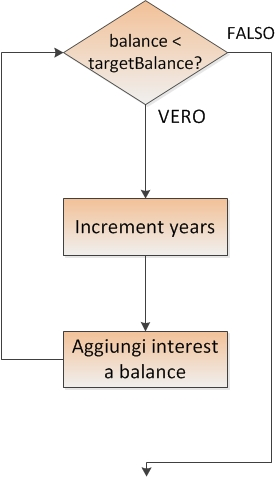
\includegraphics[scale=0.6]{images/CicloWhile.jpg}
\end{column}
\end{columns}
\end{frame}

\begin{frame}[fragile]
\begin{lstlisting}
public class Investment{
    public Investment(double aBalance, double aRate){ 
       balance = aBalance;
       rate = aRate;
       years = 0;
    }
    public void waitForBalance(double targetBalance){ 
        while (balance < targetBalance){ 
            years++;
            double interest = balance * rate / 100;
            balance = balance + interest;
        }
    }
    public double getBalance(){return balance;}
    public int getYears(){return years;}
    private double balance;
    private double rate;
    private int years;
}
\end{lstlisting}
\end{frame}

\begin{frame}[fragile]
\begin{lstlisting}
public class InvestmentTester{
    public static void main(String[] args){
        final double INITIAL_BALANCE = 10000;
        final double RATE = 5;
        Investment invest = new Investment(INITIAL_BALANCE, RATE);
        invest.waitForBalance(2 * INITIAL_BALANCE);
        int years = invest.getYears();
        System.out.println("The investment doubled after "+ years + " years");
    }
}
\end{lstlisting}
\end{frame}

\begin{frame}[fragile]
\frametitle{Cicli infiniti}
\begin{block}{}
Esistono errori logici che impediscono la terminazione di un ciclo, generando un \textbf{\alert{ciclo infinito}}
L'esecuzione del programma continua \textbf{\alert{ininterrottamente}}
\end{block}
\begin{lstlisting}
int year = 0;
while (year < 20){ 
    double interest = balance * rate / 100;
    balance = balance + interest;
}
\end{lstlisting}
\pause
\begin{lstlisting}
int year = 20;
while (year > 0){
    year++;
    double interest = balance * rate / 100;
    balance = balance + interest;
}
\end{lstlisting}
\end{frame}

\subsection*{Ciclo For}
\begin{frame}
\frametitle{Ciclo for}
\begin{block}{For al posto di while}
Molti cicli hanno questa forma:\\
\textbf{\textCl{i} = \alert{inizio;}}\\
\textbf{while(\textCl{i} $<$ \alert{fine})}\\
\textbf{$\{ \alert{enunciati}; \mbox{ } \textCl{i++}$;\}}
\end{block}
\begin{block}{Sostituzione}
\textbf{Per comodità esiste il \textbf{\textCl{ciclo for equivalente}}}\\
\hspace{0.7cm}\textbf{for(\textCl{i} = \alert{inizio}; \textCl{i} $<$ \alert{fine}; i++)}
\end{block}
\begin{block}{}
Non è necessario che l'incremento sia di una sola unità, né che sia positivo, né che sia intero.
\end{block}
\end{frame}

\begin{frame}[fragile]
\begin{block}{}
\textbf{\textCl{for(\alert{inizializzazione}; \alert{condizione}; aggiornamento)}}\\
\hspace{0.7cm} \textbf{\alert{enunciato}}
\end{block}
\begin{block}{Scopo}
Eseguire un'\textbf{\textCl{inizializzazione}}, poi \textbf{\textCl{ripetere}} l'esecuzione di un enunciato ed effettuare un 
\textbf{\textCl{aggiornamento}} finché la \textbf{\textCl{condizione}} è vera;
\end{block}
\begin{block}{Nota}
L'inizializzazione può contenere la definizione di una variabile, che \textbf{\alert{sarà visibile soltanto all'interno del ciclo}}
\end{block}
\begin{lstlisting}
for (int y = 1; y <= 10; y++){
    //corpo
}
//qui y non e' piu' definita.
\end{lstlisting}
\end{frame}